%% appendix.tex
%%

\chapter{Appendix}
\label{ch:Appendix}

\section{Autoencoder-Architekturen und Trainingsdetails}
\label{ch:Appendix:Architektur-Details}
In diesem Abschnitt werden Details zu den Autoencoder-Architekturen und Details zum Training der Autoencoder erläutert. Zuerst werden die Architekturen der klassischen vollvernetzten Autoencoder (AE), dann die Architekturen der Convolutional Autoencoder (ConvAE) und zuletzt die Architektur der Contractive Autoencoder (CAE) spezifiziert. Anschließend wird der benutzte Optimierer und andere Trainings-Details genannt. Da die Architekturen
vom Datensatz abhängen, werden diese in den folgenden Tabellen nach dem Datensatz gruppiert. Dabei steht $\text{FC}_{x}$ für eine vollvernetzte Schicht mit $x$ Neuronen. BN steht für \textit{Batch Normalization} \parencite{Ioffe.2015} und wird in vollvernetzten Autoencoder und Convolutional Autoencoder eingesetzt,
da die Autoencoder mit Batch Normalization hinsichtlich der Qualitätskriterien besser abschnitten
haben als ohne. $\text{Conv}_n$ steht für eine Convolutional Schicht mit $n$ Filter. Die
Schrittgröße wurde für alle Convolutional Schichten auf zwei gesetzt. In einem Convolutional
Autoencoder werden im Decoder Convolutional Schichten gegen Transposed Convolutional Schichten \parencite[siehe][]{Zeiler.2010} ausgetauscht. Die Schrittgröße wurde für alle Convolutional Schichten
auf zwei gesetzt.

\tabref{tab:uebersicht-autoencoder-non-image} enthält die Encoder-Architekturen der vollvernetzten und Contractive Autoencoder auf dem Swiss Roll-, Twin Peaks- und ICMR-Datensatz.
\begin{table}[ht]
	\tymax=400pt
	\tymin=200pt
	\centering
	\ra{1.3}
	\begin{tabulary}{\textwidth}{lLLLLLLL}
		\toprule
		{} & \multicolumn{3}{c}{Encoder-Architektur} \\ \cmidrule{2-4} & Swiss Roll & Twin Peaks & ICMR                                                             \\ \midrule
		AE      & $\vect{x} \in \real^3
	\newline \rightarrow \text{FC}_{5} \rightarrow \text{BN} \rightarrow \text{Sigmoid}
	\newline \rightarrow \text{FC}_{10} \rightarrow \text{BN} \rightarrow \text{Sigmoid}
	\newline \rightarrow \text{FC}_{5} \rightarrow \text{BN} \rightarrow \text{Sigmoid}
	\newline \rightarrow \text{FC}_{2} \rightarrow \text{BN} \rightarrow \text{Sigmoid}$ & $\vect{x} \in \real^3
	\newline \rightarrow \text{FC}_{3} \rightarrow \text{BN} \rightarrow \text{Sigmoid}
	\newline \rightarrow \text{FC}_{2} \rightarrow \text{BN} \rightarrow \text{Sigmoid}$ & $\vect{x} \in \real^{20531}
	\newline \rightarrow \text{FC}_{128} \rightarrow \text{BN} \rightarrow \text{Sigmoid}
	\newline \rightarrow \text{FC}_{22} \rightarrow \text{BN} \rightarrow \text{Sigmoid}$          \\ \midrule
		CAE & $\vect{x} \in \real^3
	\newline \rightarrow \text{FC}_{2} \rightarrow \text{Sigmoid}$      & $\vect{x} \in \real^3
	\newline \rightarrow \text{FC}_{10} \newline \rightarrow \text{Sigmoid}
	\newline \rightarrow \text{FC}_{2} \newline \rightarrow  \text{Sigmoid}$ & $\vect{x} \in \real^{\num{20531}}
	\newline \rightarrow \text{FC}_{22} \rightarrow \text{Sigmoid}$
		\\ \bottomrule
	\end{tabulary}
	\caption[Die Architektur des Encoders des vollvernetzten und Contractive Autoencoders für den Swiss Roll-, Twin Peaks- und ICMR-Datensatz]{Die Architektur des Encoders des vollvernetzten und Contractive Autoencoders für den Swiss Roll-, Twin Peaks- und ICMR-Datensatz. Die Architektur des Decoders ist symmetrisch zum Encoder.}
	\label{tab:uebersicht-autoencoder-non-image}
\end{table} Der Convolutional Autoencoder ist auf diesen Datensätzen nicht anwendbar und daher nicht in der Tabelle aufzufinden. Die Architekturen auf den Bilddatensätzen sind in zwei weiteren Tabellen aufgelistet. Die Architekturen für MNIST und Fashion MNIST sind in \tabref{tab:uebersicht-autoencoder-mnist}
\begin{table}[ht]
	\tymax=400pt
	\tymin=300pt
	\centering
	\ra{1.3}
	\begin{tabulary}{\textwidth}{lLL}
		\toprule
		{} & \multicolumn{2}{c}{Encoder-Architektur} \\ \cmidrule{2-3} & MNIST & Fashion MNIST                                                             \\ \midrule
		AE      & A & A \\ \midrule
		CAE & A       & A  \\ \midrule
		ConvAE & $\vect{x} \in \real^{28 \times 28} \newline
	\rightarrow \text{Conv}_{128} \rightarrow \text{BN} \rightarrow \text{ReLU} \newline
	\rightarrow \text{Conv}_{256} \rightarrow \text{BN} \rightarrow \text{ReLU} \newline
	\rightarrow \text{Conv}_{512} \rightarrow \text{BN} \rightarrow \text{ReLU} \newline
	\rightarrow \text{Conv}_{1024} \rightarrow \text{BN} \rightarrow \text{ReLU} \newline
	\rightarrow \text{Flatten} \rightarrow \text{FC}_{15}$ & $\vect{x} \in \real^{784} \newline
	\rightarrow \text{Conv}_{128} \rightarrow \text{BN} \rightarrow \text{ReLU}  \newline
	\rightarrow \text{Conv}_{256} \rightarrow \text{BN} \rightarrow \text{ReLU} \newline
	\rightarrow \text{Conv}_{512} \rightarrow \text{BN} \rightarrow \text{ReLU} \newline
	\rightarrow \text{Conv}_{1024} \rightarrow \text{BN} \rightarrow \text{ReLU} \newline
	\rightarrow \text{Flatten} \rightarrow \text{FC}_{18}$
		\\ \bottomrule
	\end{tabulary}
	\caption[Die Architektur des Encoders der Autoencoder für den MNIST und Fashion MNIST-Datensatz]{Die Architektur des Encoders der Autoencoder für den MNIST und Fashion MNIST-Datensatz. Die Architektur des Decoders ist symmetrisch zum Encoder. In einem Convolutional Autoencoder werden im Decoder Convolutional Schichten gegen Transpose Convolutional Schichten ausgetauscht. $\text{FC}_{x}$ steht für eine vollvernetzte Schicht mit $x$ Neuronen. BN steht für \textit{Batch Normalization}. $\text{Conv}_n$ steht für eine Convolutional Schicht mit $n$ Filter. Die Kernel-Größe der Convolutional Schichten beträgt $3 \times 3$ und die Schrittgröße ist zwei.}
	\label{tab:uebersicht-autoencoder}
\end{table} und für die kleineren Bilddatensätze Olivetti Faces und FER in \tabref{tab:uebersicht-autoencoder-small}.
\begin{table}[ht]
	\tymax=400pt
	\tymin=300pt
	\centering
	\ra{1.3}
	\begin{tabulary}{\textwidth}{lLL}
		\toprule
		{} & \multicolumn{2}{c}{Encoder-Architektur} \\ \cmidrule{2-3} & Olivetti Faces & FER                                                             \\ \midrule
		AE      & A & A \\ \midrule
		CAE & A       & A  \\ \midrule
		ConvAE & $\vect{x} \in \real^{28 \times 28} \newline
	\rightarrow \text{Conv}_{128} \rightarrow \text{BN} \rightarrow \text{ReLU} \newline
	\rightarrow \text{Conv}_{256} \rightarrow \text{BN} \rightarrow \text{ReLU} \newline
	\rightarrow \text{Conv}_{512} \rightarrow \text{BN} \rightarrow \text{ReLU} \newline
	\rightarrow \text{Conv}_{1024} \rightarrow \text{BN} \rightarrow \text{ReLU} \newline
	\rightarrow \text{Flatten} \rightarrow \text{FC}_{15}$ & $\vect{x} \in \real^{784} \newline
	\rightarrow \text{Conv}_{128} \rightarrow \text{BN} \rightarrow \text{ReLU}  \newline
	\rightarrow \text{Conv}_{256} \rightarrow \text{BN} \rightarrow \text{ReLU} \newline
	\rightarrow \text{Conv}_{512} \rightarrow \text{BN} \rightarrow \text{ReLU} \newline
	\rightarrow \text{Conv}_{1024} \rightarrow \text{BN} \rightarrow \text{ReLU} \newline
	\rightarrow \text{Flatten} \rightarrow \text{FC}_{18}$
		\\ \bottomrule
	\end{tabulary}
	\caption[Die Architektur des Encoders der Autoencoder für den MNIST und Fashion MNIST-Datensatz]{Die Architektur des Encoders der Autoencoder für den MNIST und Fashion MNIST-Datensatz. Die Architektur des Decoders ist symmetrisch zum Encoder.}
	\label{tab:uebersicht-autoencoder-small}
\end{table}

Alle Autoencoder benutzen das \textit{PyTorch}-Framework, wobei \textit{Skorch} für die
Kompatibilität mit anderen \textit{Scikit-Learn} Algorithmen eingesetzt wird. Als Optimierer wird
\textit{Adam} verwendet, der häufig für das Trainieren neuronaler Netze gegenüber anderen
Optimierern wie \textit{Stochastic Gradient Descent} (SGD) präferiert wird. Die Lernrate $\eta$
wird mittels eines exponentiellen Verfalls nach jeder Epoche aktualisiert. Dazu wird $\eta$ nach
jeder Epoche $t = 1, \ldots, t_{\text{max}}$ mit einem Wert $\gamma$ multipliziert. Dieser Wert
wird für alle Autoencoder auf $\gamma = \num{0,9}$ gesetzt. Der klassische Autoencoder wird für
maximal 100 Epochen, der Contractive Autoencoder für maximal 50 Epochen und die Convolutional
Autoencoder für maximal 150 Epochen trainiert. Das Training wird frühzeitig beendet, wenn sich der
Validierungsfehler innerhalb von 20 Epochen nicht mehr verbessert. Die Größe eines Batches ist
datensatzabhängig nach Stichprobengröße gewählt worden und beträgt 64 für die Swiss Roll und Twin
Peaks, 32 für Olivetti Faces und ICMR, sowie 128 für MNIST, Fashion MNIST und FER.

\section{Qualitätskriterien für die Datensätze}
\label{ch:Appendix:Qualitaetskriterien}

In diesem Abschnitt werden die Abbildungen der Qualitätskriterien für die restlichen Datensätze
gesammelt. In \figref{fig:TwinPeaksMetrics} sind die Qualitätskriterien für die Twin Peaks, in
\figref{fig:ICMRMetrics} die Qualitätskriterien für ICMR, in \figref{fig:OlivettiFacesMetrics} die
Qualitätskriterien für den Olivetti Faces Datensatz, in \figref{fig:FashionMNISTMetrics} für den
Fashion MNIST-Datensatz und in \figref{fig:FER2013Metrics} für den FER-Datensatz.
\begin{figure}[ht]
	\begin{center}
		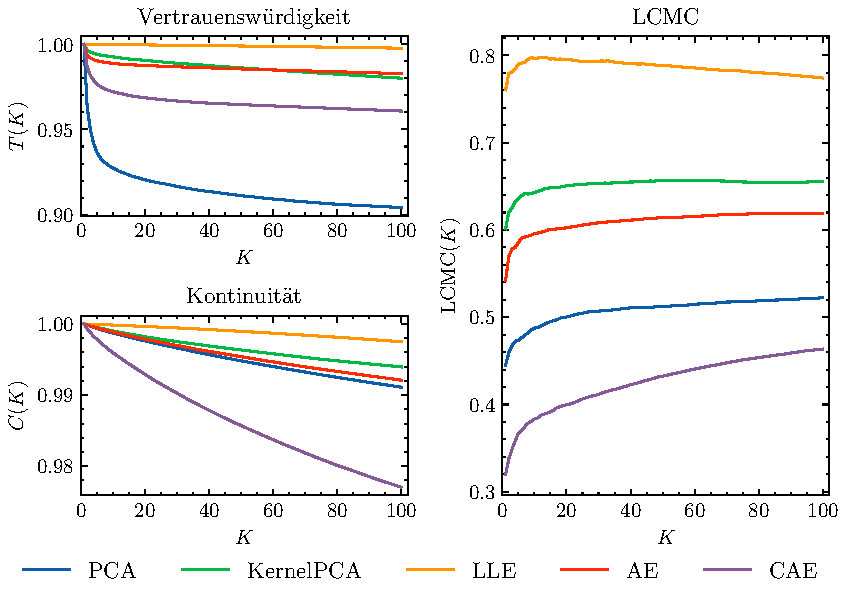
\includegraphics{TwinPeaks_comparison.pdf}
	\end{center}
	\caption[Qualitätskriterien für den Twin Peaks-Datensatz]{Die Vertrauenswürdigkeit und Kontinuität der Dimensionsreduktion, sowie das Local Continuity Meta-Criterion (LCMC) für den Twin Peaks-Datensatz. Locally Linear Embedding (LLE) schneidet wie bei der Swiss Roll insgesamt am besten ab, gefolgt von der Kernel PCA und vom Autoencoder. Lediglich der Contractive Autoencoder (CAE) und PCA fallen auf diesem künstlichen Datensatz etwas zurück, wobei die Vertrauenswürdigkeit der Dimensionsreduktion von PCA deutlich schlechter als bei den restlichen Methoden ist. Dies ist wahrscheinlich der nichtlinearen Mannigfaltigkeit geschuldet, was der linearen Principal Component Analysis Schwierigkeiten bereitet. (Eigene Darstellung)}
	\label{fig:TwinPeaksMetrics}
\end{figure}

\begin{figure}[ht]
	\begin{center}
		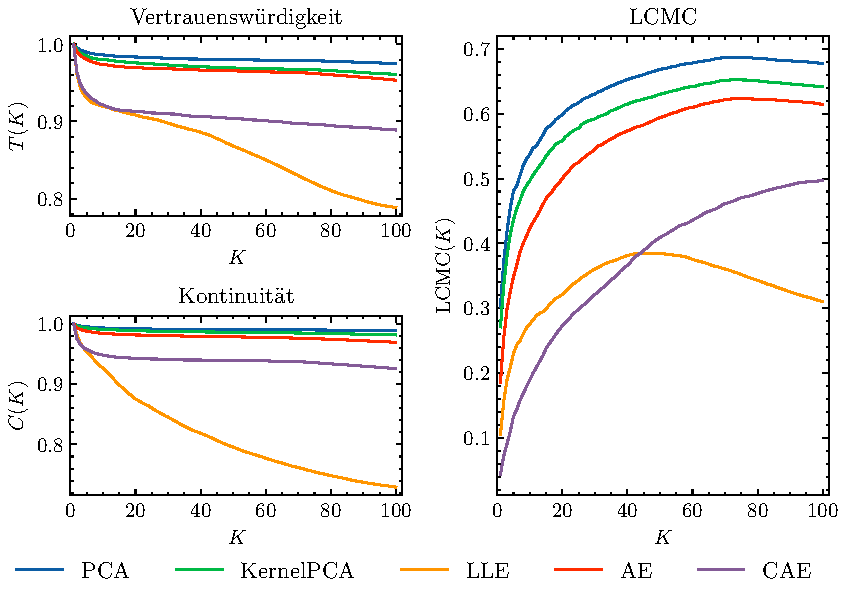
\includegraphics{ICMR_comparison.pdf}
	\end{center}
	\caption[Qualitätskriterien für den ICMR-Datensatz]{Die Vertrauenswürdigkeit und Kontinuität der Dimensionsreduktion, sowie das Local Continuity Meta-Criterion (LCMC) für den ICMR-Datensatz. Dieser Datensatz ist kein Bilddatensatz, weswegen hier der Convolutional Autoencoder nicht eingesetzt werden konnte. Hier schneidet die Principal Component Analysis am besten ab, gefolgt von der Kernel PCA und vom vollvernetzten Autoencoder. Am schlechtesten sind der Contractive Autoencoder und Locally Linear Embedding, wobei die Qualitätskriterien mit größer werdender Nachbarschaftsgröße $K$ bei LLE deutlicher abfallen. (Eigene Darstellung)}
	\label{fig:ICMRMetrics}
\end{figure}

\begin{figure}[ht]
	\begin{center}
		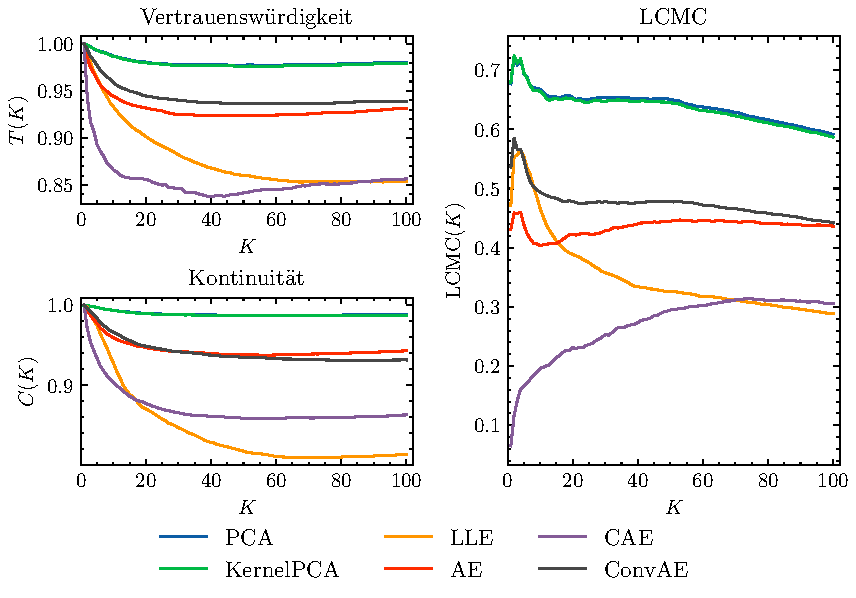
\includegraphics{OlivettiFaces_comparison.pdf}
	\end{center}
	\caption[Qualitätskriterien für den Olivetti Faces-Datensatz]{Die Vertrauenswürdigkeit und Kontinuität der Dimensionsreduktion, sowie das Local Continuity Meta-Criterion (LCMC) für den Olivetti Faces Datensatz. Principal Component Analysis und die nichtlineare Erweiterung Kernel PCA sind auf diesem Datensatz fast identisch und liefern gleichzeitig die besten Ergebnisse auf allen drei Kriterien. Alle Varianten der Autoencoder fallen hier etwas in der Performance ab. Dies könnte an der geringen Stichprobengröße von 400 liegen, wodurch eine Konvergenz der Autoencoder schwieriger wird. Neben den Autoencoder schneidet hier auch LLE für größere Werte von $K$ schlecht ab, kann jedoch bei geringeren Nachbarschaftsgrößen noch gute Werte für die drei Kriterien erreichen. (Eigene Darstellung)}
	\label{fig:OlivettiFacesMetrics}
\end{figure}

\begin{figure}[ht]
	\begin{center}
		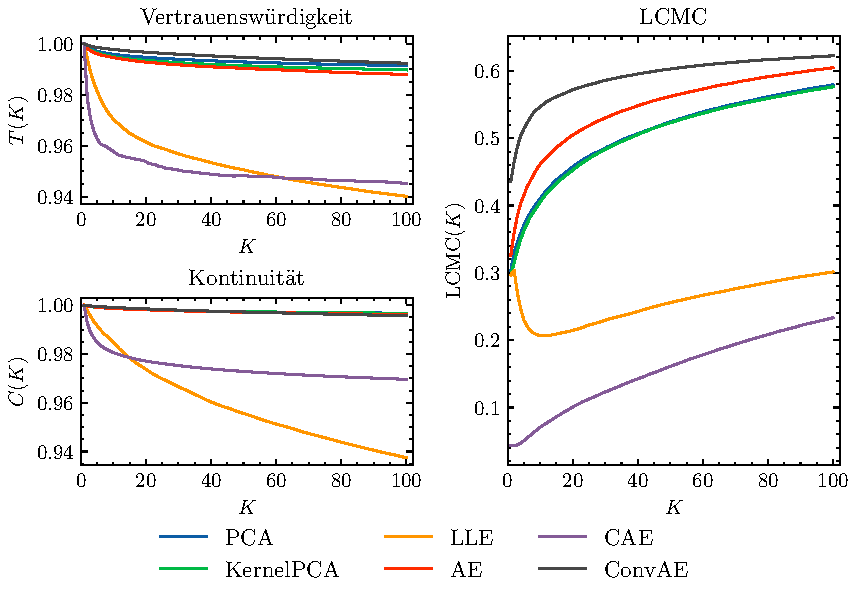
\includegraphics{FashionMNIST_comparison.pdf}
	\end{center}
	\caption[Qualitätskriterien für den Fashion MNIST-Datensatz]{Die Vertrauenswürdigkeit und Kontinuität der Dimensionsreduktion, sowie das Local Continuity Meta-Criterion (LCMC) für den Fashion MNIST-Datensatz. Die Kriterien auf diesem Datensatz zeigen ein ähnliches Bild wie auf dem Fashion MNIST-Datensatz, jedoch können die Principal Component Analysis, Kernel Principal Component Analysis und der Autoencoder etwas näher aufschließen. Alle Methoden bis auf Locally Linear Embedding und der Contractive Autoencoder können eine fast perfekte Vertrauenswürdigkeit und Kontinuität erreichen. Hinsichtlich des LCMC schneidet der Convolutional Autoencoder am besten ab, gefolgt vom vollvernetzten Autoencoder, sowie von PCA und Kernel PCA. (Eigene Darstellung)}
	\label{fig:FashionMNISTMetrics}
\end{figure}

\begin{figure}[ht]
	\begin{center}
		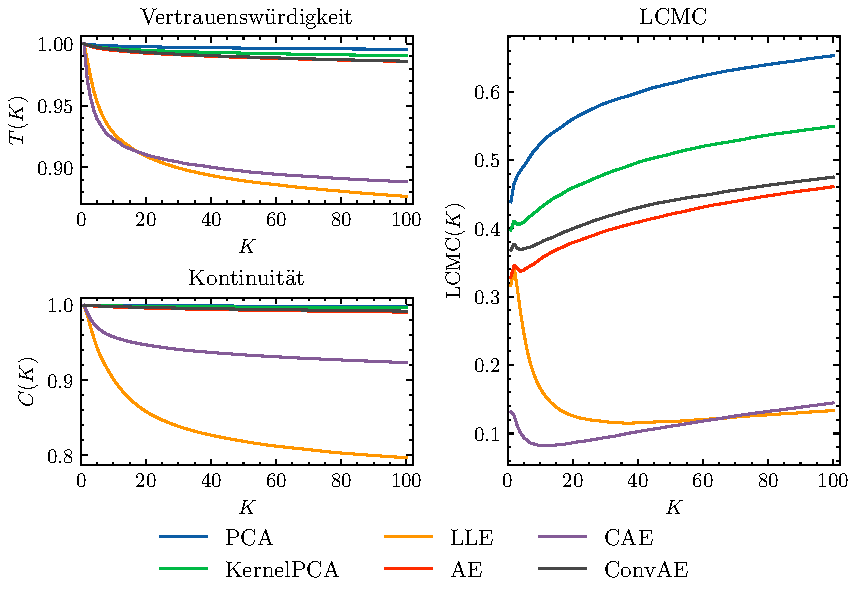
\includegraphics{FER2013_comparison.pdf}
	\end{center}
	\caption[Qualitätskriterien für den FER-Datensatz]{Die Vertrauenswürdigkeit und Kontinuität der Dimensionsreduktion, sowie das Local Continuity Meta-Criterion (LCMC) für den FER-Datensatz. Hier ist die Performance des Convolutional Autoencoders und des vollvernetzten Autoencoders nahezu identisch. Aber auch der Autoencoder und die Kernel PCA können einen konstant hohen Wert für $T(K)$ und $C(K)$ erreichen. Auch auf diesem Datensatz schneiden LLE und der Contractive Autoencoder mit Abstand am schlechtesten ab. Besonders LLE zeigt hier die Schwäche einer lokalen Erhaltung der Struktur, da die Qualitätskriterien für steigende Werte von $K$ stark abfallen. (Eigene Darstellung)}
	\label{fig:FER2013Metrics}
\end{figure}

% \section{Sonstige Abbildungen}

% \begin{figure}
% 	\centering
% 	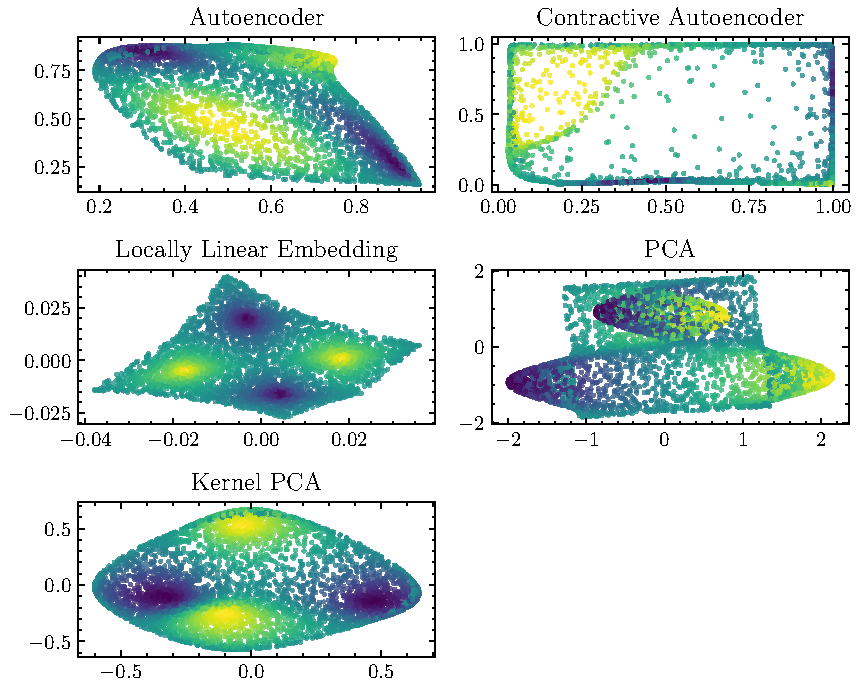
\includegraphics{TwinPeaksEmbeddings.pdf}
% 	\caption[Latente zweidimensionale Repräsentationen $\mat{Y}$ durch Anwendungen fünf unterschiedlicher Methoden auf dem Twin Peaks-Datensatz.]{Abgebildet sind die latenten zweidimensionalen Repräsentationen $\mat{Y}$ durch Anwendungen fünf unterschiedlicher Methoden auf dem Twin Peaks-Datensatz. Die von Locally Linear Embedding gefundene latente Repräsentation hat die einzelnen Peaks herabsenken können. Kernel PCA konnte dies im Gegensatz zur linearen Principal Component Analysis ebenfalls erkennen. Auch die latente Repräsentation des vollvernetzten Autoencoders zeigt diesen Ansatz, verzerrt die Peaks in der Ebene jedoch stärker als es bei LLE oder Kernel PCA der Fall ist. Der Contractive Autoencoder scheint alle Punkte auf die Ränder abzubilden, was die niedrigere Vertrauenswürdigkeit und Kontinuität erklärt.}
% 	\label{fig:TwinPeaksEmbeddings}
% \end{figure}